\chapter{绪论}
%这是-连字符
\normalspacedchars{-}%为了正确表示连字符,为了看效果可以注释掉本句,然后取消上下两句的注释,作用区域是本宏指令之后的内容,包括在绪论之后的其他章节
%这是-连字符
\section{多智能体系统概述}
\subsection{多智能体系统研究背景}
使得整个群体表现出单个个体所不能达到的行为的内在规律,并且将这些内部工作机制及理论应用到实际中\scite{couzin2002collective};物理学家们则希望运用更为精确的数学模型,通过计算机模拟这些现象并且能够深入直观地解释这些令人讶异的群体行为\scite{tanner2003stable,程代展2004从群集到社会行为控制};另外在控制科学领域,\cite{洪奕光2011多智能体系统动态协调与分布式控制设计,olfati2007consensus,savkin2004coordinated}提出了很有意义的研究方向。
\subsection{智能体系统简介}
智能体的研究起源于20世纪70年代初,文本文本文本。
\subsection{多智能体系统一致性问题研究现状}
除了上面提到的Boid 和Vicsek 两个经典模型,下面列举几种常见的多智能体动力学模型及其控制协议的设计。

对于以下的一阶连续积分器动力学模型:(无编号公式)
\[\dot{x}_i=u_i, i=1,2,\ldots,n,
\]
其中,$x_i\in R^n$是第$i$个智能体的位置状态,$u_i\in R^n$表示施加的控制输入。对于这样的单积分器系统,学者们设计了不同的控制协议(有编号公式),
\begin{equation}
u_i=-\sum_{j\in N_i(t)}a_{ij}(t)(x_i(t)-x_j(t)),
\end{equation}

图\ref{formation}展示了几种多智能体系统编队控制在一些领域的应用。
\begin{figure*}[H]
\begin{centering}
\subfloat[多机器人世界杯足球锦标赛]
{
\begin{centering}
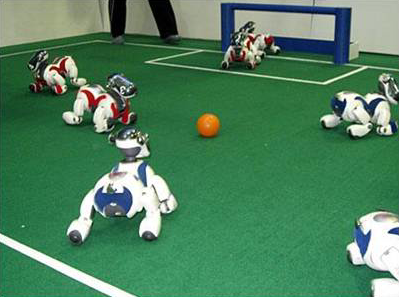
\includegraphics[width=0.45\textwidth]{1.png}
\end{centering}
}
\subfloat[无人机编队]
{
\begin{centering}
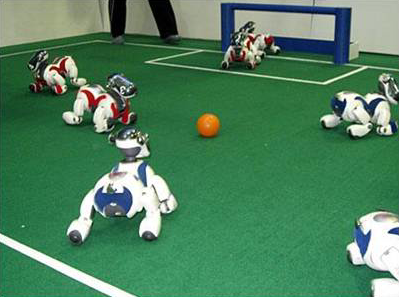
\includegraphics[width=0.45\textwidth]{1.png}
\end{centering}
}
\end{centering}
\\
\begin{centering}
\subfloat[多个机械手臂协同作业]
{
\begin{centering}
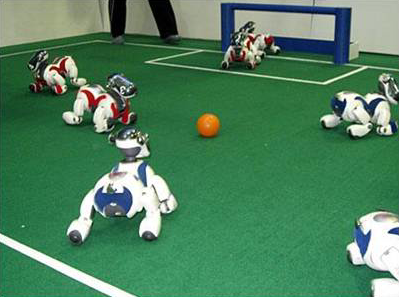
\includegraphics[width=0.45\textwidth]{1.png}
\end{centering}
}
\subfloat[城市交通控制管理系统]
{
\begin{centering}
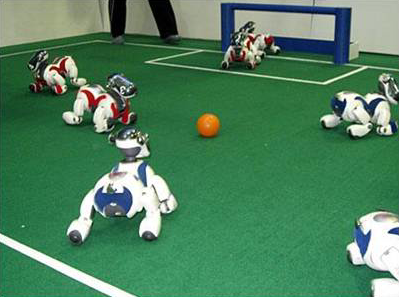
\includegraphics[width=0.45\textwidth]{1.png}
\end{centering}
}
\end{centering}
\protect\caption{多智能体系统编队控制在实际中的应用}
\label{formation}
\end{figure*}
